\chapter{Performance Modeling of Sparse Factorization Solvers}

%{\color{blue} juraj: introduction to performance modelling: know the max performance limit before doing further optimizations, what is the hw utilization of the code?}

Performance engineering plays an important role in development of scientific software. In order to achieve optimal performance, one needs to analyze the code and computer architecture to identify bottlenecks and possibilities for optimization (\cite{KöstlerRüde+2013+91+96,Minami2019}). This helps us spend our effort only where there is a potential for improvement.
%It is also useful to have realistic expectations about performance given code can achieve.
While simple code can be often analyzed using intuition and guessing, this is not possible for nontrivial codes. Performance models are helping us to analyze a code by guiding our attention on important features and neglecting unnecessary details~(\cite{Gropp99,Williams:EECS-2008-164,KHWPAF14}).
%
%In this chapter we analyze forward and backward substitution code used in direct methods for solving sparse linear systems. Due to the fact that part of the algorithm is executed sequentially and part in parallel, the performance predictions are challenging. With our extension to the roofline model we are able to model such code. The predictions are then compared to measurements for a representative set of sparse matrices.
%
%Last, the Execution-Cache-Memory (ECM) model is studied as a theoretical base for use for modeling of forward and backward substitution \todol{in the next chapter}.
%Unlike the roofline model, ECM takes into account deep knowledge of the computer architecture, in particular in-core execution and cache hierarchy, which might allow it more accurate predictions.
%
This chapter reviews two performance models we will later use for modeling forward and backward substitution code used in sparse factorization solvers.

The chapter is organized as follows. In Section \ref{sec:arch} computer architecture is briefly introduced. Next, Section \ref{sec:likwid} reviews a collection of command line tools called LIKWID. These tools are useful for various performance engineering tasks, e.g. determining the hardware and its specification, micro-benchmarking and profiling. After that, two established performance models are reviewed: Berkeley Roofline model in Section \ref{sec:roofline} and Erlangen Execution-cache-memory model in Section \ref{sec:ecm}. Finally in Section \ref{sec:ecm-application} Execution-cache-memory model is used to analyze performance of two simple computational kernels. Models of these two kernels will be later used as a base for modeling sparse triangular solve.

%\section{Code parameters}
%
%\subsection*{Work}
%
%With $W$ we denote work. It is the number of operations executed by a program or algorithm. It could refer to any type of operation, but here we always measure work in floating point operations (FLOPs) in double precision.
%We don't count instructions because one instruction can perform more than one floating point operation.
%
%In kernels like dot product, there is often multiplication followed by addition. To make these computations more efficient, many modern CPU architectures compute operations similar to $a=a+b*c$ in one instruction. This type of instructions is called fused multiply-add (FMA).
%Other widely used computation is applying the same operation on many operands, vector addition $A[:]=B[:]+C[:]$. This is in hardware implemented using so called vector instructions. Advanced Vector Extensions (AVX) operates on registers of size 256\,b, which can store 4 operands in double precision or 8 in single precision. One AVX instruction performs 4 FLOPs. And AVX2 adds support of vectorized FMA operations, so 8 FLOPs are performed in a single instruction.
%
%\subsection*{Performance}
%
%Performance refers to number of operations per unit of time.
%If program finishes performs $W$ operations and finishes the computations in time $T$, then it achieves performance $P = W/T$.
%
%\subsection*{Memory traffic}
%
%Before processor can perform computations, data has to be loaded to registers. The data has to travel form memory to the L3 cache, then to L2 and L1 and finally to the registers. The registers and cache have very limited size, so after the computations when the data are not needed anymore, it has to travel through the hierarchy back to memory.
%
%We denote the data transferred from memory to L3 cache $Q_r$ (read) and the data transferred from L3 cache to memory $Q_w$ (write), all measured in bytes. The memory traffic is $Q = Q_r + Q_w$.
%We could also examine traffic between different cache levels, but for the memory traffic we are interested only in the data transferred between memory and the L3 cache.
%
%\subsection*{Operational intensity and code balance}
%
%The operational intensity is a ratio between work and memory traffic $I = W / Q$, number of floating point operations for 1\,B or memory transfer.
%Similar to operational intensity is arithmetic intensity, but it is defined as \todol{todo}.
%
%Sometimes it is more convenient using code balance instead of operational intensity. This is defined as $B_c = I^{-1} = Q / W$, number of bytes per one floating point operation.
%
%\section{Machine parameters}
%
%\subsection*{Peak performance}
%
%Peak performance is theoretical maximum the processor is designed to compute. To achieve the peak performance, the processor must utilize all cores and in every cycle it executes the instructions that compute the most operations. Typically these are the AVX (4 FLOPs/cycle) or AVX2 instructions (8 FLOPs/cycle).
%As and example let's look at an Intel Xeon E5-2695 v3. This is a 14 core CPU with Haswell architecture and frequency 2.3\.GHz. The Haswell architecture supports AVX2 and can execute two instructions per cycle.
%So the peak performance is $P_{peak} = 2.3 * 14 * 8 * 2 = 515.2\,\textrm{GFLOPs/s}$.
%Evaluation of the peak performance of modern CPUs is not as easy as it seems. It depends on an instruction set and number and type of units in a core. Nice analysis of different Intel architectures can be found in \cite{dolbeau-2018}.
%
%However, the peak performance is a theoretical maximum that most real world applications are not able to achieve.
%For example if compiler cannot vectorize the code, the performance drops by factor of four. And if a kernel uses only addition or only multiplication, for example sum of elements in a vector, then the performance drops to a half.
%Instead of peak performance we use attainable performance, denoted as $P_{max}$. This allows more realistic expectations based on knowledge of the code and instructions set used by the compiler.
%
%\subsection*{Memory bandwidth}
%
%Memory bandwidth $b_s$ is a rate at which data can be read and stored into memory.
%The bandwidth found in a datasheet does not have to be reachable by the app, similar to the peak performance.
%The memory bandwidth depends on access pattern, number of threads, if NUMA is used and Cluster-on-Die\footnote{Cluster-on-Die (CoD) solves a problem with saturation of memory bandwidth on server CPUs from Intel. These CPUs have many cores (14 or more), but only few can are able to saturate the memory bandwidth. When CoD is enabled, the cores, memory and L3 cache are split to two NUMA domains and second memory controller is used. This reduces the number of cores using the same memory controller and doubles the memory bandwidth.} enabled.
%More realistic bandwidth can be obtained using micro-benchmark, ideally with similar memory access pattern as the application.
%
%\subsection*{Machine balance}
%
%Machine balance $B_m = b_s / P_{max}$ is a ratio of memory bandwidth and attainable performance.
%If $B_c < B_m$ then the code’s performance is limited by the max performance, it is compute bound. Optimizing memory access of such code does not improve performance. One should focus on optimizing computations, for example using vector instructions as much as possible.
%If $B_c > B_m$ then the code’s performance is limited by the memory bandwidth, hence it is memory bound. Here performance can be improved by optimizing memory access pattern, for example by reusing data loaded to cache us much as possible, so they don't have to be loaded from memory.

\section[Memory Hierarchies, Autotuning, and Solvers]{Exploiting the Memory Hierarchies, Autotuning\\ Research, and Sparse Factorization Solvers}
\label{sec:modeling-intro}

Modern microprocessors are highly sensitive to the spatial and temporal locality of data. Regardless of the programming model, performance of future parallel applications will crucially depend on the quality of the generated code which is traditionally the responsibility of the compiler. The compiler selects which optimization to perform in terms of, e.g., loop-unrolling, out-of-order instruction capabilities, or register scheduling. Choosing parameters for these optimizations, and selecting among alternative implementations, is the key to efficient use of the underlying hardware. The resulting space of optimization alternative is large (\cite{8423171}).

Autotuner projects such as, e.g. ATLAS~\footnote{Automatically Tuned Linear Algebra Software} (\cite{whaley04,WN147}), FLAME~\footnote{Formal Linear Algebra Methods Environment} (\cite{Flame:2005}), and OSKI~\footnote{Optimized Sparse Kernel Interface} (\cite{Demmel2005:selftune:linalg,Vuduc2003:thesis,Lee2004:spmv:symm}),
gained popularity as a very effective approach for producing high-quality portable scientific code. In these projects, the set of library kernels is automatically optimized by generating many variants of a given kernel and by running that kernel in a target platform. The search process may take hours to complete on the platform. However, it needs to be performed only once when the library is installed on the platform. The resulting codes might be
several times faster than naive implementations.

As an example, reordering the vertices and elements in a mesh can have a significant impact on performance. Graph and hypergraph techniques have been used in this area to automatically generate highly efficient, platform-adapted implementations of {\sl sparse matrix kernels}. These kernels are frequently computational bottlenecks in diverse applications in computational science and engineering applications. However, the task of extracting near-peak performance on modern cache-based superscalar machines has proven to be extremely difficult. Many sparse matrices from applications have a natural block structure that can be exploited by storing columns as a collection of blocks and thus accelerating the performance of sparse matrix kernels significantly. It is shown in recent projects such as \cite{BEBOP2016,Vuduc2003:thesis} that it is possible to build an automatic tuning system to generate implementations whose performances exceed that of the best hand-tuned code. The algorithmic methods behind these research projects are based on reordering methods on the discrete graph structure in order to maximize the block structure and, thus, obtaining high performance by maximizing spatial and temporal locality.
%\enlargethispage*{\baselineskip}

\section{Computer architecture}
\label{sec:arch}

%\todop{
%+ cores
%+ ports (image)
%+ out of order !!!!!
%+ instrucitons (pipeline, Haswell, ...)
%+ AVX
%+ FMA
%+ NUMA
%+ CoD
%+ Peak performance (all together)
%+ Memory bandwidth
%}

Modern processors utilize numerous techniques that aim to improve performance --- the number of computations done per unit of time. In the past, the performance used to be increased only by increasing the CPU clock frequency. However, increasing the frequency results in higher power consumption and, consequently, the CPU needs a larger heat sink in order to prevent it from overheating. As a result, the clock frequency of recent CPUs is about 2.0--3.5\,GHz and does not increase anymore.
Since the trend of doing computations faster due to increasing frequency is over, the effort of CPU manufacturers focuses on performing computations at the same time in parallel.
This leads to adding more computational units to modern processors. These units, called cores, perform instructions independently, thus the overall performance is effectively increased. This scheme works well when every core works on different data, but when an access to shared data is required the cores need to be synchronized in order to prevent data conflicts and inconsistent results. The synchronization, however, requires serialization of computation and prevention parallel computations, thus reducing the overall performance.

Another possibility for parallel computations is implementing instructions that perform more than one operation applied on vectors of data instead of single elements. Such instructions are called SIMD (Single Instruction Multiple Data), examples of which are SSE (Streaming SIMD Extensions) that operates on 128\,b registers containing two floating point numbers in double precision or four numbers in single precision, or newer AVX (Advanced Vector Extensions) with registers twice as big, computing four operations in double precision in a single instruction.

Another CPU optimization focuses on computational pattern, where there is multiplication followed by addition. An example of such an operation can be found in many compute kernels in various scientific applications. In order to make these computations more efficient, many modern CPU architectures compute operations similar to $a=a+b*c$ in one instruction. This type of instruction is called fused multiply-add (FMA).
The new version of an AVX extension, called AVX2, adds support for vectorized FMA operations, effectively performing 8 operations in a single instruction using double precision (16 operations in single precision).

\begin{figure}[t]
  \centering
  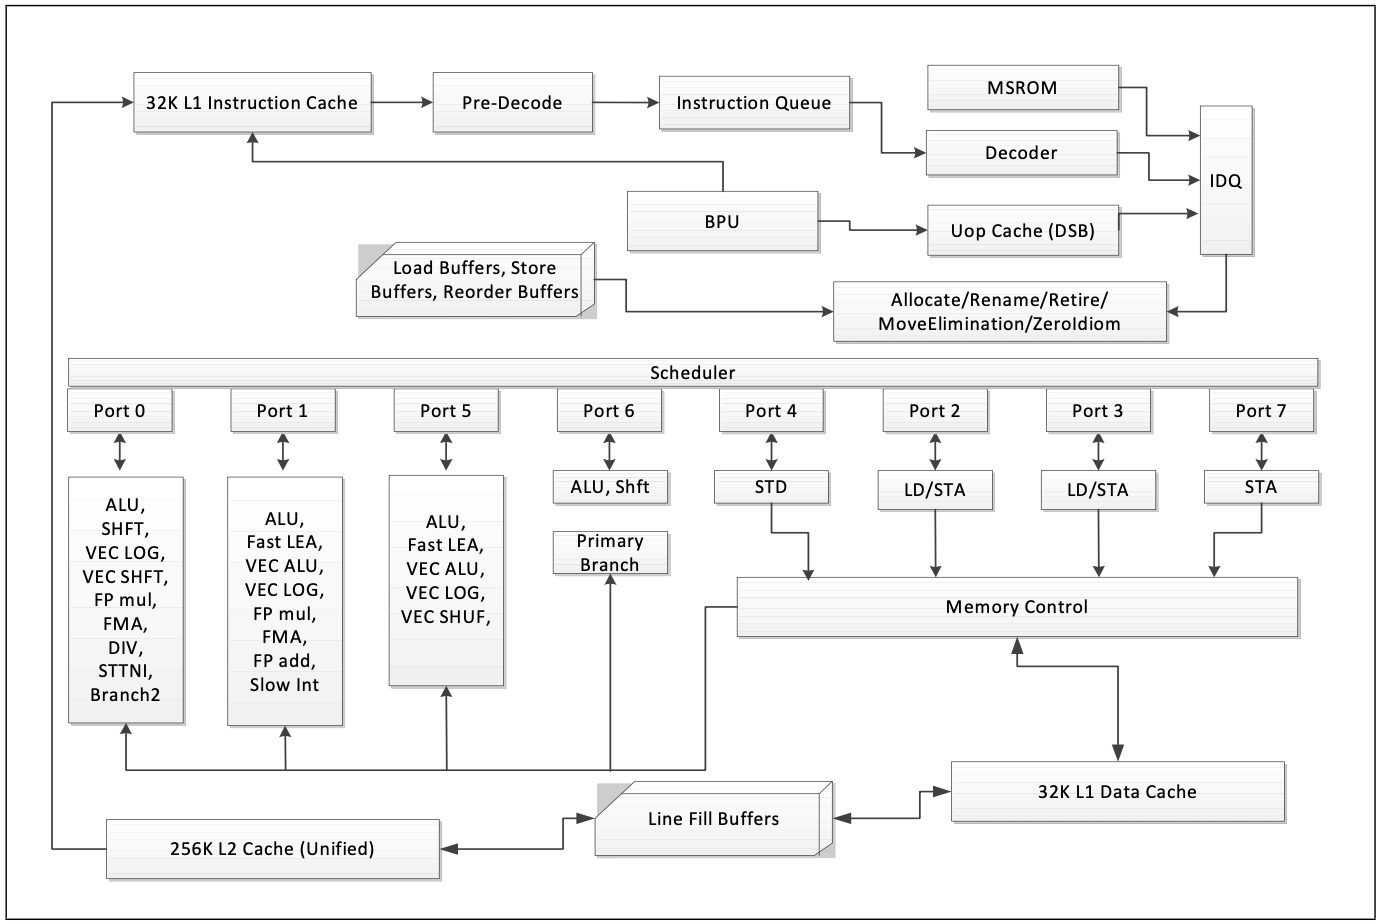
\includegraphics[width=\textwidth]{images/haswell_microarchitecture.png}
  \caption{CPU core pipeline of Haswell microarchitecture. From \cite{intel-orm-2016}.}
  \label{fig:hsw-microarch}
\end{figure}

The parallelism can be exploited not only on the level of multiple cores, but also on the instruction-level within a single processor, an example of which is instruction pipelining. Pipelining attempts to divide incoming instructions into a series of sequential steps, allowing the processor to dispatch a new instruction every cycle, instead of performing a whole instruction which takes several cycles. Additionally, in order to maximize instruction throughput, the instructions are executed out of order, if there are available processing units.
A CPU core of Intel Haswell microarchitecture is shown in Figure \ref{fig:hsw-microarch}, consisting of eight dispatch ports in total, four of which have units for computational operations and four for memory operations. The scheduler can dispatch up to eight micro-ops every cycle, one on each port.

Another level of complexity is introduced when considering data movements. The CPU performs all operations on data stored in registers, the fast but small memory inside the CPU. Before the computations start, data have to first be loaded from memory to registers and when the computations are done, they have to be stored back to memory. The memory is very slow compared to the registers, which introduces a significant bottleneck hampering the performance of a computation. To make the memory access more efficient there are multiple levels of memory between the CPU and main memory, each with different size and access speed, referred to as cache. Usually the cache has three levels, called L1, L2, and L3. L1 is closest to the CPU and has the smallest size (few kB), while L3 is closest to the memory and has the largest size (few MB). Any data transferred between the memory and registers have to go through all cache levels. 
In some cases data are often reused in the computation, thus they can stay in the cache, avoiding communication with the slow memory.

In order to improve performance and the ability of the system to be expanded, e.g., in the case of servers often having more than one processor, every processor has its own memory and memory controller. This memory layout is called NUMA (Non-Uniform Memory Access). The benefit of such an architecture is that it increases memory bandwidth, the rate at which data can be read and stored into memory, which prevents a~bottleneck introduced by all the cores accessing the memory and saturating the available bandwidth, resulting in idle cores waiting for data instead of doing useful computation. On the other hand, introducing multiple memory domains creates problems when one processor needs to access data in memory belonging to another processor. This situation is possible but not very efficient, as it increases the load at a single memory controller and, additionally, the data have to be transferred through a link between processors, which can become a bottleneck. The programmer works with a virtual memory spanning all memory domains, so he does not see this underlying complexity, but he should keep this in mind in order to write efficient code. For example, an operating system places memory pages to the physical memory of the processor that writes to the page for the first time, so called first touch. If a single thread initializes all the data that are then accessed in parallel, it might allocate the data in a suboptimal way. If the initialization is performed in parallel, significantly better memory utilization can be achieved.

\begin{table*}[t]
%\parbox{.7\linewidth}{
  \footnotesize
 \centering
%\resizebox{\textwidth}{!}{%
 \begin{tabular}{p{1.9cm}llrrrrrrrrr}
    \hline
    name      & &  & IVB         & HSW-D      & HSW-S           & BDW           & SKX         & KNL           & ZEN-D        &  ZEN-S         \\
    \hline
    \multirow{3}{\linewidth}{processor name} & &  & Intel& Intel & Intel & Intel & Intel & Intel & AMD &  AMD \\
      & &  & Xeon  & Xeon & Xeon      & Xeon    & Xeon  & Xeon    &
~~Ryzen 7   &  ~~EPYC      \\
              & &  &\scriptsize  E5-2660 v2 &\scriptsize  E3-1240 v3
&\scriptsize  E5-2695 v3      &\scriptsize  E5-2630 v4    &\scriptsize  Gold
6148   &\scriptsize  Phi 7210      &\scriptsize  1700X      &\scriptsize
745           \\
%     processor & &  & Intel Xeon  & Intel Xeon & Intel Xeon      & Intel Xeon    & Intel Xeon  & Intel Xeon    & AMD Ryzen    &  AMD EPYC      \\
%     name      & &  &  E5-2660 v2 & E3-1240 v3 & E5-2695 v3      & E5-2630 v4    & Gold 6148   & Phi 7210      & 7 1700X      &  745           \\
    \hline
    micro     & &  & Ivy Bridge  & Haswell    & Haswell         & Broadwell
& Skylake     & ~Knigths       & Zen          &  Zen           \\
    arch.     & &  &             &            &                 &               &             & Landing       & \\
    \hline
    freq    & [GHz] & & 2.2      & 3.4        & 2.3             & 2.2           & 2.4         & $\approx$ 1.3 & 3.4          &  2.3           \\
    cores   &       & & 10       & 4          & 2 $\times$ 7    & 10            & 20          & 64            &   8          &  24            \\
    ISA     &       & & AVX      & AVX2       & AVX2            & AVX2          & AVX-512     & AVX-512       & AVX2         &  AVX2          \\
%    sockets &       & 2        & 1          & 2               & 2             & 2           & 1             & 1            &  & 1 \\
%    \mltwo{NUMA LDs}& 2        & 1          & 2 $\times$ 2    & 2 $\times$ 2  & 2           & 1             & 1            &  & 1 \\
    \mltwo{NUMA LDs} & & 1       & 1          & 2               & 1             & 1           & 1             & 1            & 4              \\
    \hline
    L1 & [KiB]     &  &  32      & 32         & 32              & 32            & 32          & 32            & 32           &  32            \\
    L2 & [KiB]     &  &  256     & 256        & 256             & 256           & 1024        & 1024          & 512          &  512           \\
    L3 & [MiB]     &  &  25      & 8          & 2 $\times$ 17.5 & 25            & 28          & -             & 2 $\times$ 8 &  8 $\times$ 8 \\
    \hline
%    copy bw. & [GB/s] & 41.2   & 26.6            & 22.6       & 31.3 & ?? &  75.9 & 30.2 & 212 \\ % complete socket/cod
%    read bw. & [GB/s] & 44.3   & 30.9            & 23.6       & 33.7 & ?? &  74.2 & 32.5 & 231 \\ % complete socket/cod
    \mlfour{scalar read bw.}   &     &          &  \\
    ~1 core  & [GB/s]  &&  9.5 & 16.6 & 12.1 & 11.5 &  14.5 &  8.5 & 19.3 & 19.3  \\
    ~NUMA LD & [GB/s]  && 44.4 & 22.7 & 31.2 & 56.3 & 108.0 & 75.2 & 33.7 & 37.6  \\
    \hline
    \mlfour{scalar ADD+MUL/FMA} &&& \\
    ~1 core  & [F/cy] &&  2 &  4 &  4 &  4 &  4 &   4 &  4 &  4 \\
    ~NUMA LD & [F/cy] && 20 & 16 & 28 & 40 & 80 & 256 & 32 & 24 \\
    \hline
    \mlfour{scalar machine balance $B_m$} &  &         & \\
    ~1 core  & [B/F] && 2.2 & 1.2 & 1.3 & 1.3 & 1.5 & 1.6 & 1.4 & 2.1 \\
    ~NUMA LD & [B/F] && 1.0 & 0.4 & 0.5 & 0.6 & 0.6 & 0.2 & 0.3 & 0.7 \\
    \hline
\\[0.01em]
  \end{tabular}
  \caption{Details of Evaluated Hardware Systems.
% ISA Lists the Latest Extension Supported by the Processor.
% Read Memory Bandwidth, Floating Point Instructions per Cycle (ADD+MULL and
% FMA Instructions), and Machine Balance is Reported for Scalar Execution.
KNL's Bandwidth Numbers are for DDR Memory.}
% ECM: 2 cy L1/L2 bei HSW/BDW entgegen der Doku
% STREAM:
% read = summation
% KNL: no-nt, prefetch not explicitly disabled
% ZEN: no-nt, AVX2, only even cores
% HSW2: no-nt, avx2
% HSW: no-nt, avx2
% IVB: no-nt,
  \label{tab:hw}
%} % from https://tex.stackexchange.com/a/27105
%}
\end{table*}

Modern server processors contain a lot of cores (usually 14 or more) and with so many cores accessing the memory it is very easy to saturate the memory bandwidth. Intel solves this problem by splitting the memory and L3 cache between two NUMA domains and use second memory controller. This reduces the number of cores using the same memory controller and doubles the memory bandwidth. Intel calls this architecture Cluster-on-Die (CoD).
%Cluster-on-Die (CoD) solves a problem with saturation of memory bandwidth on server CPUs from Intel. These CPUs have many cores (14 or more), but only few can are able to saturate the memory bandwidth. When CoD is enabled, the cores, memory and L3 cache are split to two NUMA domains and second memory controller is used. This reduces the number of cores using the same memory controller and doubles the memory bandwidth.

Peak performance of a CPU is a theoretical maximum the processor can\linebreak achieve. It requires utilization of all cores running at the base frequency and every core achieving the highest possible floating point throughput.
Evaluation of the peak performance of modern CPUs is a very intricate process, requiring one to consider a multitude of factors. It depends on an instruction set and the number and type of units in a core. A detailed analysis of different Intel architectures can be found in \cite{dolbeau-2018}.
As an example we can analyze Intel Xeon E5-2695 v3. This is a 14 core CPU with Haswell architecture and base frequency 2.3\,GHz (detailed description is in Table \ref{tab:hw}). The Haswell architecture supports AVX2 instructions (8 FLOPs per instruction) and can execute two instructions per cycle (ports 1 and 5), resulting in a total of 16 FLOPs per cycle per core.
Consequently, the peak performance is $P_{peak} = 2.3 * 14 * 8 * 2 = 515.2\,\textrm{GFLOPs/s}$.

The theoretical memory bandwidth can be found in a datasheet, but the attainable bandwidth of a specific application depends on the access patters, number of threads used, whether NUMA is used, and other factors. Using the theoretical bandwidth is thus not precise for purposes of performance analysis.
A more realistic bandwidth can be obtained using microbenchmarks, ideally with similar memory access patterns as the application.
%\texttt{likwid-bench} from the LIKWID toolbox is a popular application for benchmarking different kernels.
In the following section we will review a performance tool called LIKWID which supports software developers, benchmarkers and application users to model and get the best performance on a given system. We will use this tool later for performance modeling for a sparse factorization solver.

\section{Performance modeling using the LIKWID Tools}
\label{sec:likwid}

LIKWID ("Like I Knew What I'm Doing") (\cite{likwid-2010-arxiv}) is set of command line tools to support optimization and performance engineering.
It consists of tools that display thread and cache topology, discover CPU and memory performance using benchmarks, alter CPU frequency and other settings, and allow performance evaluation of user applications.
Typical workflow using the LIKWID tools could be (i) use \texttt{likwid-topology} to find information about the hardware, (ii) gather various performance metrics using \texttt{likwid-bench} (memory bandwidth, performance using different instruction sets, etc.). Next, (iii) run an application specifying thread affinity using \texttt{likwid-pin} and (iv) evaluate performance a of user application using \texttt{likwid-perfctr} by collecing performance metrics either for the whole runtime or only for a specified code region.
A short description of the most useful tools follows.

\subsection*{likwid-topology}

Performance engineering requires  in-depth knowledge about node topology, like NUMA domains, cache hierarchy and sizes, CPU architecture, frequency, cores, and HW threads.
This information can be gathered using various command line tools, which might be time consuming, especially since some of them present long output where it is difficult to find required information. \texttt{likwid-topology} provides a holistic picture of node topology, collecting information from different available sources in the operating system and presenting a comprehensive and easy to understand overview of the node topology either in intuitive text form or an ASCII art style.

\subsection*{likwid-pin}

Thread affinity is crucial for performance of scientific applications. Knowing the topology (obtained, for example, by \texttt{likwid-topology}), one can pin threads to cores according to the application's requirements.
Pinning threads make performance measurements more consistent between runs and usually also improve performance bacause the threads are not assigned to cores randomly. This is very important when multiple NUMA domains are used to minimize the data traffic between NUMA domains.
%
\texttt{likwid-pin} can be used with all applications based on POSIX threads, which include most of OpenMP implementations. The pinning is achieved by overloading the \texttt{pthread\_create} call and pinning every thread upon creation.
Some OpenMP implementations create shepherd threads. These threads do not execute any user code and therefore should not be pinned. This is achieved by providing a mask or using one of the predefined masks for known implementations.

\subsection*{likwid-perfctr}

All modern CPUs provide hardware counters, registers that can be set to count various hardware events. The main purpose of these counters is to help manufacturers with development of the CPU, but they are also available to the user. The counters are accessed using model specific registers (MSR) and can be configured to count various events like fetching data, storing data, cache hits/misses, or calculations. As the counters are implemented in hardware, they come with no overhead. A downside of using the counters is that they measure events on a given core and cannot distinguish between processes. However, on systems with only one user this is usually not a problem.

\texttt{likwid-perfctr} is a command line tool that configures and reads the counters and is used as a wrapper for a user application.
It can be used in two modes: it can either measure the whole runtime of the application or only specific blocks of code called regions.
If the whole runtime is measured, no modification of the application is needed.
For measuring the regions, markers denoting the beginning and end of a region have to be inserted into the application code and have to be linked with the likwid library. The markers are library function calls that read values of the counters. 
Every marker has a name (user defined string) identifying the region. The string does not have to be unique, but all regions with the same name are summed up and are indistinguishable in the output. 
After the user application finishes, the data from counters are processed and a summary is presented. As reading the counters is a simple operation and all the processing is done after the user app finishes, there is very little overhead.

The measured events are specified as command line arguments to the wrapper application, so the measurement can be repeated several times measuring different events without recompiling the code.
The raw counts usually do not provide a lot of insight. However, \texttt{likwid-perfctr} can combine the raw counts to derive useful performance metrics like FLOPs/s or memory bandwidth.
%
Additionally, \texttt{likwid-perfctr} has also functionality of \texttt{likwid-pin}. This is very important because without pinning the threads could move between cores, making the measurements inaccurate.
\enlargethispage*{\baselineskip}

\subsection*{likwid-bench}

Writing a benchmark is a very intricate process. The purpose of a benchmark is to measure some specific computation; however, the naive user code might not necessarily be the most efficient implementation. A compiler exploits a lot of optimizations, e.g., if results of some computations are not used, these computations are often dropped altogether. Alternatively, a compiler can replace the user code by more efficient implementation. In both cases, the benchmark would end up measuring something different from what was intended.
To be sure the benchmark measures the proper thing, the code most likely has to be written in assembly or at least the user should check the assembly generated by a compiler.

\texttt{likwid-bench} is a benchmark suite for prototyping low-level assembly kernels. 
It contains a set of various kernels, for example, dot product, daxpy, load, store, copy, and many others. It allows the user to define his own kernels. The kernels are defined as text files that are compiled during compilation of the suite. And the suite takes care of everything else: running the kernel on a problem of a given size, on a given number of threads, and presenting results to the user.

\section[Berkeley Roofline model]{Berkeley Roofline model - A Performance Model for Multicore Architectures}
\label{sec:roofline}

Programmers often do not need an understanding of every detail of CPU design. They should focus on general concepts rather than details of every available architecture. A tool that can provide a simplified model of the CPU hiding most of the architecture specific complexity is very valuable. Probably the most popular tool was popularized by \cite{williams-2009}. This tool is called the Roofline model.
It became very popular because it hides most of the CPU complexity and presents an intuitive and easy to use model that can guide performance engineering.
This model has proven to be useful not only on the most common architecture, x86\_64, where it was extended to address cache hierarchy (\cite{MARQUES2020257}), but it was successfully used also on other architectures, e.\,g., ARM, an architecture developed for battery powered devices, where power efficiency is the biggest concern, but since then it found its way to desktop computers and even the most powerful supercomputers~(\cite{9307836}); GPU accelerators, where (\cite{9059264,https://doi.org/10.1002/cpe.5547}); Intel Xeon Phi (\cite{10.1007/978-3-319-32149-3_12}) and even FPGA~(\cite{9307865}). Moreover it was also used for modeling energy consumption (\cite{6569852}).

%\todop{
%abstraction, hides detais (ports, ...)
%easy to use
%two bottlenecks
%shows maximum performance given code can achieve, useful when compared with measurements, we can see how far the measured performance is from the theoretical maximum
%}

The model analyzes bottlenecks during execution on a given hardware.
A compute kernel reads data from memory, does some computations, and writes the results back to memory. Let's denote $W$ as the size of data read or written to memory in Bytes and $F$ the number of operations the kernel computes. Usually we are interested in floating point operations (FLOPs), additions and multiplications, but we could generalize this to any kind of operations.
Let's assume the machine has peak performance $P_{peak}$ measured in [FLOPs/s] and peak memory bandwidth $b_s$ measured in [B/s].
It is reasonable to expect the processor needs $F/P_{peak}$\,s to finish all computations and it needs $W/b_s$\,s for the memory transfer (reading and writing data). If we assume the computation and memory transfer can perfectly overlap, the total runtime is equal to the one that take longer:
\begin{equation}
    T = \max(F/P_{peak}, W/b_s).
\end{equation}

Working with runtime is not very useful because it depends on the size of the problem. Instead we usually compare performance $P=F/T$ [FLOPs/s].
Let's also define arithmetic intensity as the number of operations per one byte of memory transfer, $I=F/W$. Then we can write the expected performance as
\begin{equation}
   P = min(P_{peak}, I \cdot b_s). \label{eq:roofline}
\end{equation}

Sometimes it is easier working with code balance instead of arithmetic intensity. Let's define code balance as the number of transferred bytes per one operation, $B_c=W/F=I^{-1}$. Then we can write (\ref{eq:roofline}) as
\begin{equation}
   P = min(P_{peak}, b_s/B_c). \label{eq:roofline_balance}
\end{equation}

\begin{figure}[t]
   \centering
   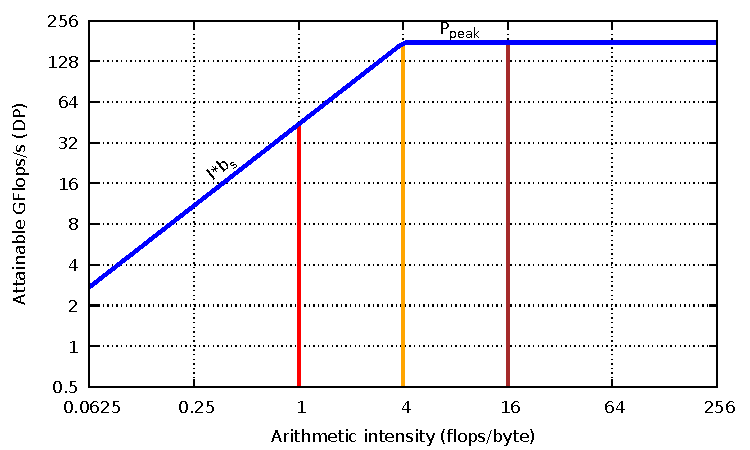
\includegraphics[width=0.7\textwidth,clip=true]{images/roofline/roofline_emmy_Xeon2660v2_naive.pdf}
   \caption{Roofline model of Intel Xeon E5-2660 v2 (blue) and three generic kernels (red, orange, and brown).}
  \label{fig:roofline_emmy_naive}
\end{figure}

We can see a graphical representation of (\ref{eq:roofline}) in Figure \ref{fig:roofline_emmy_naive} in a blue color. The shape of the graph looks like a roof, which gives the model its name.
The performance bound increases with increasing arithmetic intensity until it saturates at the peak performance. This happens where the two lines corresponding to the two bottlenecks intersect. The arithmetic intensity of this intersection equals $P_{peak}/b_s$ or machine balance $B_m=b_s/P_{peak}$. We call it machine balance and not code balance because it characterizes the machine.

In Figure \ref{fig:roofline_emmy_naive} we can also see three vertical lines. These lines represent three generic kernels with arithmetic intensity 1, 4, and 16. We can expect the performance of these kernels somewhere along the respective lines.
Note that the lines are below the roofline, since the roofline is the performance upper bound.
The red kernel (arithmetic intensity 1) is in the bandwidth limited region. The performance is increasing with increasing arithmetic intensity. Looking at the intersection of the red and blue line, we can expect a performance bound of approximately 44\,GFLOPs/s.
The brown kernel (arithmetic intensity 16) is in the compute bound region. With increasing arithmetic intensity the memory traffic decreases, but the performance does not increase.
And the orange kernel (arithmetic intensity $4 \approx B_m^{-1}$) is between these regions. Performance of this kernel depends on machine ability to overlap computation and memory communication (loads and stores).

%Machine balance $B_m = b_s / P_{max}$ is a ratio of memory bandwidth and attainable performance.
%If $B_c < B_m$ then the code’s performance is limited by the max performance, it is compute bound. Optimizing memory access of such code does not improve performance. One should focus on optimizing computations, for example using vector instructions as much as possible.
%If $B_c > B_m$ then the code’s performance is limited by the memory bandwidth, hence it is memory bound. Here performance can be improved by optimizing memory access pattern, for example by reusing data loaded to cache us much as possible, so they don't have to be loaded from memory.

%The point where the two lines intersect is at operational intensity $I = B_m^{-1}$. At this point the performance $P_{max}$ is achieved while reading and writing to memory as much as possible, $b_s$\,B/s.
%Performance of any kernel on the right side of this point ($B_c < B_m$ or $I > B_m^{-1}$) is limited by $P_{max}$. We call such kernel compute bound.
%Performance of any kernel on the left side of this point ($B_c > B_m$ or $I < B_m^{-1}$) is limited by $b_s$. We call such kernel memory bound.

\subsection{Roofline Ceilings}

For realistic applications the measured performance of a kernel is often far below the roofline. The CPU and memory architecture utilize several paradigms that improve the performance, as described in section \ref{sec:arch}. To get close to the maximum performance the kernel needs to exploit these. Failing to do so results in a huge performance penalty.
For both bounds the roofline model takes into account, in-core execution and memory bandwidth, we can show ceilings showing impact on performance when certain optimizations are not implemented.

\subsubsection*{In-core Roofline Ceilings}

%\todop{
%vectorization
%data dependencies (pipeline, vectorization)
%FMA
%}

As discussed in section \ref{sec:arch} processors achieve peak performance when all cores are utilized and all of them are using only the instructions that perform the most operations. These are usually the vector instructions AVX on Haswell architecture and newer AVX2 (FMA operation applied on a vector).
If the compiler is unable to use these instructions, it comes with a huge penalty in performance. If scalar instructions are used, only 1/4 of peak performance can be achieved. If FMA is not used, performance drops to 1/2. And if neither AVX nor FMA is used, then we can expect only 1/8 of peak performance.

%In kernels like dot product, there is often multiplication followed by addition. To make these computations more efficient, many modern CPU architectures compute operations similar to $a=a+b*c$ in one instruction. This type of instructions is called fused multiply-add (FMA).
%Other widely used computation is applying the same operation on many operands, vector addition $A[:]=B[:]+C[:]$. This is in hardware implemented using so called vector instructions. Advanced Vector Extensions (AVX) operates on registers of size 256\,b, which can store 4 operands in double precision or 8 in single precision. One AVX instruction performs 4 FLOPs. And AVX2 adds support of vectorized FMA operations, so 8 FLOPs are performed in a single instruction.

For example, the following code snippet computes sum of elements in a vector.
\begin{algorithmic}[1]
  %\State sum = 0.0
  \For{i = 0; i < n; i++}
      \State sum += a[i]
  \EndFor
\end{algorithmic}%
It may seem this code cannot be vectorized because it would cause write conflicts in the variable \texttt{sum}.
But the compiler can transform this code introducing new variables.
\begin{algorithmic}[1]
  %\State sum = 0.0
  \For{i = 0; i < n; i+=4}
      \State sum0 += a[i    ]
      \State sum1 += a[i + 1]
      \State sum2 += a[i + 2]
      \State sum3 += a[i + 3]
  \EndFor
\end{algorithmic}%
In this code there are no dependencies anymore, so it can be vectorized.
This means the four consecutive elements from the array fit in a 256\,b AVX register and the same for the sum variables. Then AVX instruction computes all four operations at the same time, achieving 4 FLOPs per instruction.

Another example is a prefix sum.
In this case there are loop-carried dependencies preventing vectorization.
\begin{algorithmic}[1]
  \For{i = 1; i < n-1; i++}
      \State a[i] += a[i-1]
  \EndFor
\end{algorithmic}%

So while in the first case the loop can be vectorized and achieve 4 FLOPs/instruction, in the second example vectorization is not possible, achieving only 1 FLOP/instruction with scalar instructions.
Note that both algorithms use only additions and no multiplications, so FMA is not used. As a result the best performance one could expect is $P_{peak}/2$ for the first code and $P_{peak}/8$ for the second one.
Visualization of some in-core ceilings is given in Figure \ref{fig:roofline_emmy_core-ceilings}.
%\todol{Not all ceilings are shown in this graph, for example the ceiling with AVX and without FMA (like in the first code snippet) is missing.}

\begin{figure}[t]
   \centering
   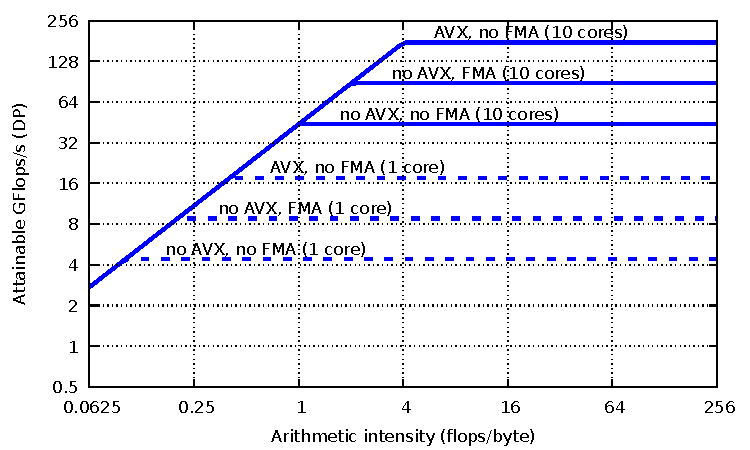
\includegraphics[width=0.7\textwidth,clip=true]{images/roofline/roofline_emmy_Xeon2660v2_core-ceilings.pdf}
   \caption{Berkeley Roofline model of Intel Xeon E5-2660 v2 with various in-core ceilings for 1 and 10 cores.}
  \label{fig:roofline_emmy_core-ceilings}
\end{figure}

\subsubsection*{Bandwidth Roofline Ceilings}

%\todop{
%prefetching?
%}

In Figure \ref{fig:mrm:bw-scaling} we can see memory bandwidth achieved by two Haswell processors (desktop and server) using a different number of cores. The desktop processor nearly saturates the bandwidth with one core, but the server processor achieves only about 40\% of bandwidth with a single core and needs at least 3 or 4 cores to fully saturate the bandwidth.

When data are transferred between memory and the L3 cache or different cache levels, they are always transferred in chunks called cache line. On Intel processors the size of cache line is usually 64\,B. Even if only 1\,B is needed, the whole cache line is transferred. Or when data are accessed with nonunit stride, some data are transferred and not used. This can lead to saturating the memory bandwidth while getting little useful data.

When NUMA is used, there is a memory controller at every NUMA domain. If all data are allocated on the same controller, this can happen, for example, by wrong first touch (initializing the data sequentially), then the other controllers are not used, lowering the bandwidth. Also when processes from one domain access data from another domain, the communication goes through a NUMA link between domains, which can become a bottleneck.

In Figure \ref{fig:roofline_emmy_memory-ceilings} we can see the effect of lower bandwidth when single core is used on the roofline model. As the bandwidth is lower, the corresponding line moves down. Note also the intersection of the horizontal and skewed line. It moved from arithmetic intensity 4\,F/B to about 16\,F/B, so a kernel that is compute bound on 10 cores could become memory bound on 1 core.

\begin{figure}[t]
   \centering
   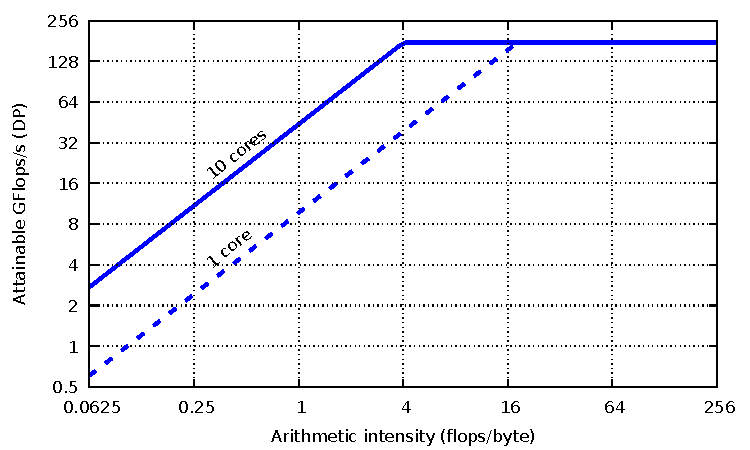
\includegraphics[width=0.7\textwidth,clip=true]{images/roofline/roofline_emmy_Xeon2660v2_memory-ceilings.pdf}
   \caption{Roofline model of Intel Xeon E5-2660 v2 with bandwidth ceilings for 1 and 10 cores.}
  \label{fig:roofline_emmy_memory-ceilings}
\end{figure}

As it is not possible reading data from memory using one thread and using all available threads for computations or vice versa, we can combine Figures \ref{fig:roofline_emmy_core-ceilings} and \ref{fig:roofline_emmy_memory-ceilings}. The roofline model with both in-core and bandwidth ceilings is shown in Figure \ref{fig:roofline_emmy_all-ceilings}.

\begin{figure}[t]
   \centering
   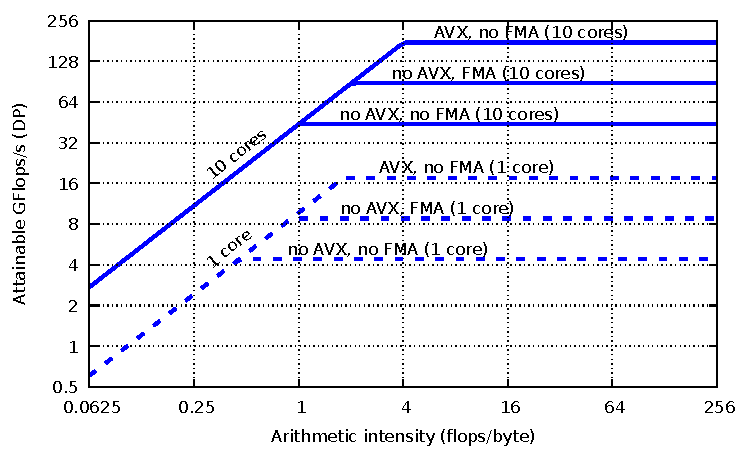
\includegraphics[width=0.7\textwidth,clip=true]{images/roofline/roofline_emmy_Xeon2660v2_all-ceilings.pdf}
   \caption{Roofline model of Intel Xeon E5-2660 v2 with both in-core and bandwidth ceilings.}
  \label{fig:roofline_emmy_all-ceilings}
\end{figure}

\begin{figure*}%
  \centering%
  
 \begin{tabular}{cc}
 %\begin{tabular}{>{\tiny \bfseries}lcccccccccc>{\tiny \bfseries}lccccccccccc}
 \multicolumn{1}{c}{\tiny \bfseries IVB} & \multicolumn{1}{c}{\tiny \bfseries
HSW-D} \\
  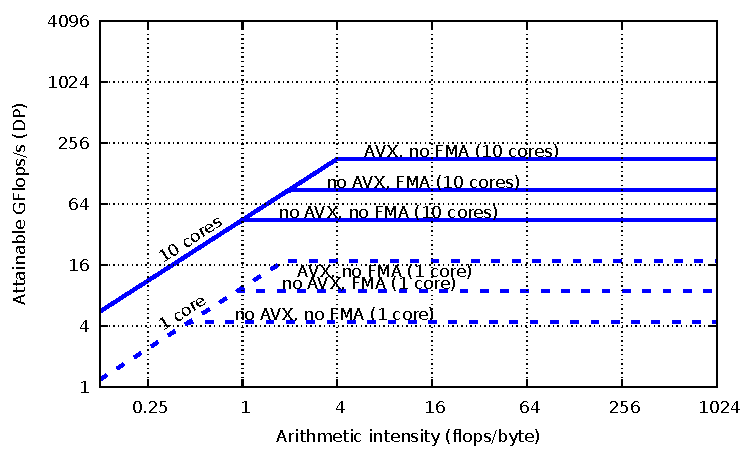
\includegraphics[width=0.49\textwidth,clip=true]{images/roofline/roofline_IVB.pdf}% 
  & 
  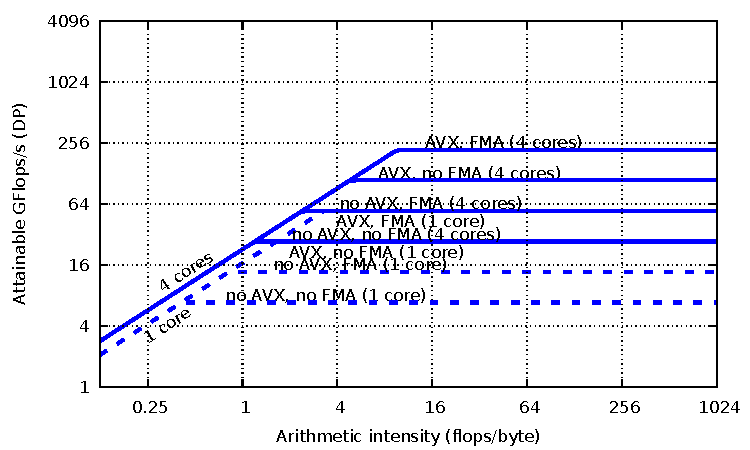
\includegraphics[width=0.49\textwidth,clip=true]{images/roofline/roofline_HSW-D.pdf}% 
  \\
  
\multicolumn{1}{c}{\tiny \bfseries HSW-S} & \multicolumn{1}{c}{\tiny
\bfseries BDW} \\
  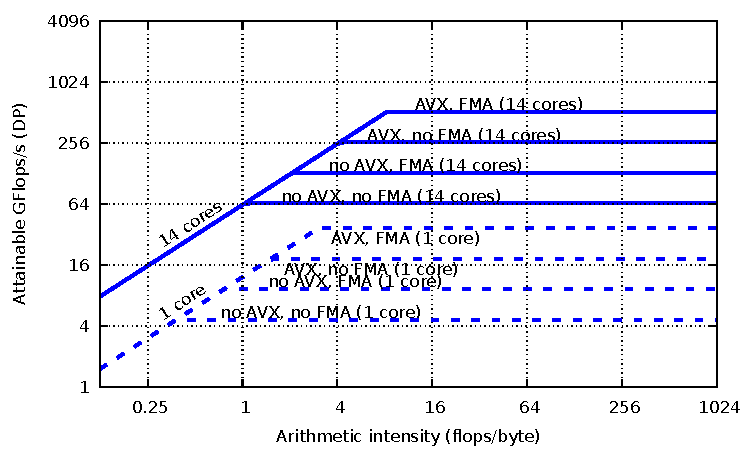
\includegraphics[width=0.49\textwidth,clip=true]{images/roofline/roofline_HSW-S.pdf}% 
  & 
  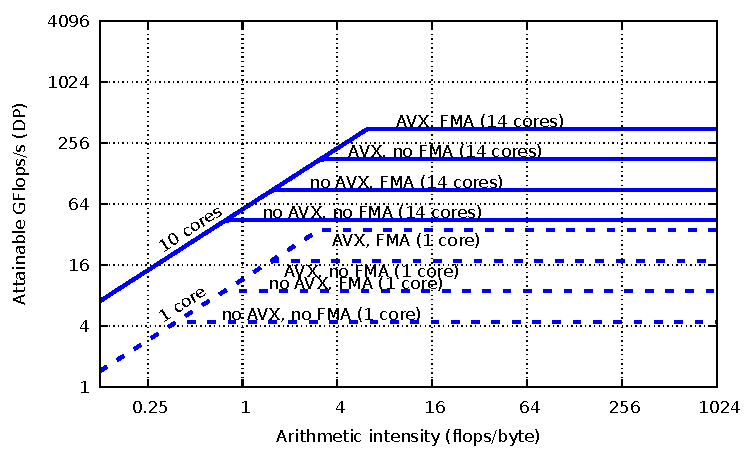
\includegraphics[width=0.49\textwidth,clip=true]{images/roofline/roofline_BDW.pdf}% 
  \\
  
\multicolumn{1}{c}{\tiny \bfseries SKX} &
\multicolumn{1}{c}{\tiny \bfseries KNL} \\
  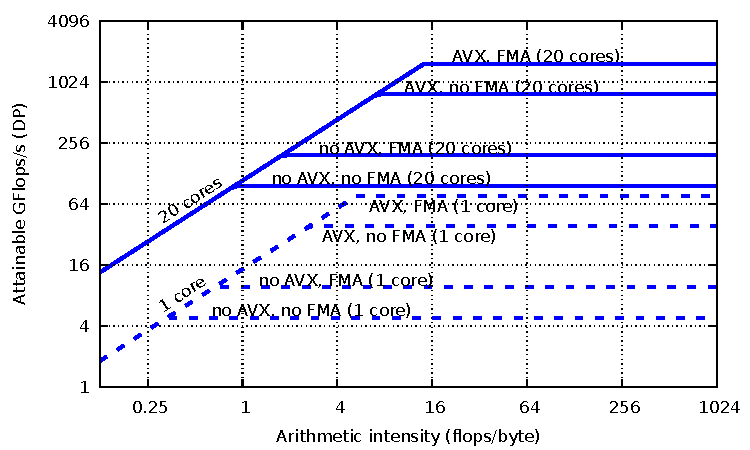
\includegraphics[width=0.49\textwidth,clip=true]{images/roofline/roofline_SKX.pdf}% 
  & 
  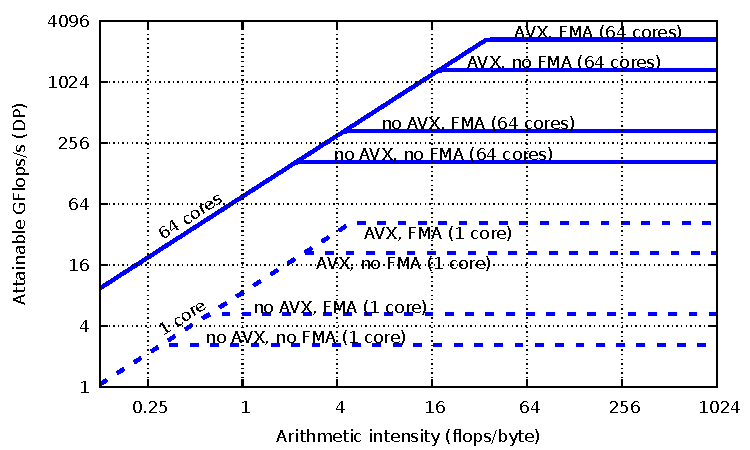
\includegraphics[width=0.49\textwidth,clip=true]{images/roofline/roofline_KNL.pdf}% 
  \\
  
\multicolumn{1}{c}{\tiny \bfseries
ZEN-D} & \multicolumn{1}{c}{\tiny \bfseries ZEN-S} \\
  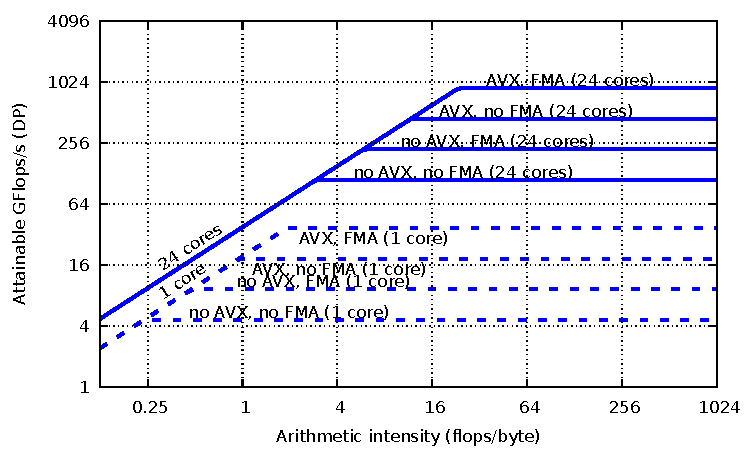
\includegraphics[width=0.49\textwidth,clip=true]{images/roofline/roofline_ZEN-S.pdf}% 
  & 
  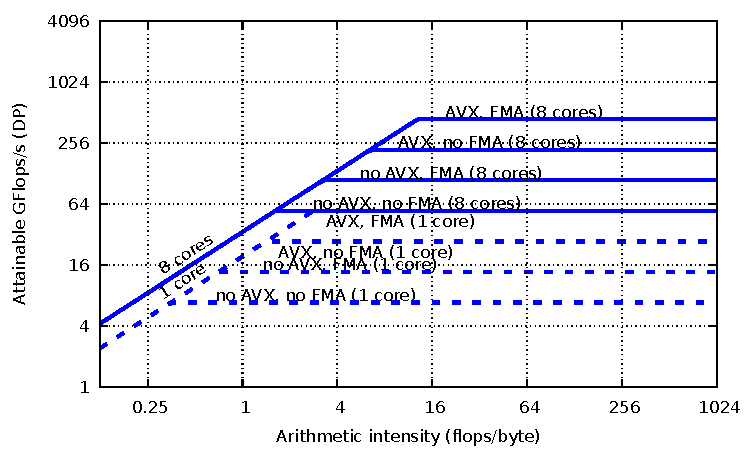
\includegraphics[width=0.49\textwidth,clip=true]{images/roofline/roofline_ZEN-D.pdf}% 
\\

\end{tabular}
%%
  %
  \caption{Roofline models of processors listed in Table \ref{tab:m:list}.}%
  \label{fig:rooflines}
\end{figure*}

%The Roofline model brings together two machine parameters describing possible bottlenecks, maximum performance $P_{max}$ and memory bandwidth $b_s$, and visualizes upper bound of performance any code can achieve on given machine.
%It is a graph with operational intensity $I$ on the x-axis and performance $P$ on the y-axis. The two bottlenecks are displayed as two lines:
%The horizontal line is a visualizaiton of attainable performance $P = P_{max}$.
%The skewed line is a function of memory bandwidth and operational intensity $P = I * P_{max}$.
%As these are the factors limiting the performance, we can expect performance of any program must be below these lines or in the best case on the lower of the two limits.
%We can write the performance upper bound as a function of either operational intensity or code balance as
%\begin{equation}
%   P = min(P_{max}, I \cdot b_s) = min(P_{max}, b_s / B_c).
%\end{equation}
%This can be visualized as \todol{ref naive graph}.
%The shape of the graph is what gives the model its name.
%
%Any compute kernel can be shown in the graph as a vertical line under the roofline. X-coordinate of the line is the operational intensity of the kernel.
%We can expect the performance of given kernel is somewhere along this line. Closer to the roofline (higher) is better, but the it can never exceed the roofline.
%
%The point where the two lines intersect is at operational intensity $I = B_m^{-1}$. At this point the performance $P_{max}$ is achieved while reading and writing to memory as much as possible, $b_s$\,B/s.
%Performance of any kernel on the right side of this point ($B_c < B_m$ or $I > B_m^{-1}$) is limited by $P_{max}$. We call such kernel compute bound.
%Performance of any kernel on the left side of this point ($B_c > B_m$ or $I < B_m^{-1}$) is limited by $b_s$. We call such kernel memory bound.
%
%%\todop{
%%\begin{itemize}
%%    \item naive, ceilings
%%    \item cite williams
%%\end{itemize}
%%}
%
%\begin{figure}[H]
%   \centering
%   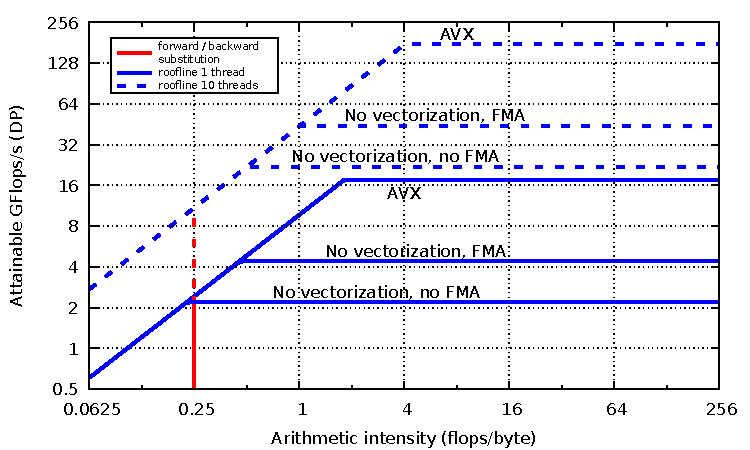
\includegraphics[width=0.7\textwidth,clip=true]{images/roofline_emmy_Xeon2660v2}
%   \caption{Roofline model of the  Intel Xeon E5-2660 v2 CPU.}
%  \label{fig:roofline_emmy}
%\end{figure}
%
%
%%\todop{
%%\begin{itemize}
%%    \item Description of CPU
%%    \item Memory hierarchy
%%\end{itemize}
%%}

\section{Erlangen Execution-cache-memory model}
\label{sec:ecm}

The Roofline model is a simple model
for performance prediction in the saturated case.
Hereby it is assumed code is limited by floating point performance or by the
memory bandwidth.
The ECM performance model (\cite{treibig-2010-ecm,hager-2012-ecm}) is a refinement
of the Roofline model.\footnote{For further details regarding the ECM model refer
to~\cite{stengel-2015}.}
In contrast it allows a performance prediction on the single core level as well
as a scaling prediction over the socket.
The model takes into account the duration of the code execution inside the core
separated by arithmetic and data movement.
Furthermore data transfers in the memory/cache hierarchy are considered as well
as the achievable memory bandwidth.
%
Finally both parts build the single core model, which is used to determine the
scaling behavior over the cores until a bottleneck is reached. 
%
For memory bound codes this is typically the achievable memory bandwidth, as all
other infrastructures like Intel's L3 cache on Ivy Bridge, Haswell, and Broadwell
scale perfectly. 

The ECM model has some restrictions on the code to be analyzed.
It is important that streaming accesses are performed. This means prefetching
works perfectly and can hide latency effects.
The ECM model predicts the number of CPU cycles (cy) required to execute a certain number of iterations of a given loop on a single core. Since the smallest amount of data transferred between cache levels is one cache line (CL), it is a reasonable unit of work for the predictions. The size of cache line on Intel processors is 64\,B, which is for streaming kernels 8 iterations with floating point numbers in double precision.

To construct the model, we consider two parts separately: the in-core execution, assuming all data were already fetched to the L1 cache and there are no cache misses, and the time to fetch the data from its location to the L1 cache.
 %the main memory or the cache level where it is assumed to be stored

\subsection*{In-core execution}

To determine the in-core execution time, a simple model for instruction throughput on the given architecture is required. Figure \ref{fig:hsw-microarch} shows a port model for the Intel Haswell architecture. The port scheduler schedules instructions to ports independently out of program order, making sure all data dependencies are met.

Instructions inside ports are pipelined, but only one instruction per port can
be issued per cycle.
Haswell can perform two loads (LD, ports~$2D$ and~$3D$) and one store (ST,
port~$4$) of sizes up to $32$\,B at the same time (\cite{intel-orm-2016}), each.
Each load and store requires an address to be generated by an address
generation unit (AGU, ports~$2$,~$3$, and~$7$).
However on port~$7$ only a simple AGU is located, which is limited to simple
addressing modes\footnote{AGUs on port 2 and 3 support addressing "base plus index plus offset", AGU on port 7 supports only simple addressing mode "base plus offset".}~(\cite{intel-orm-2016,hofmann-2016-hsw}).
%
For floating point operations, the cores host two 
FMA units (port~$0$ and~$1$), two multiplication (MUL) units (port~$0$
and~$1$), and one add (ADD) unit (port~$1$).

For the ECM model the duration of the execution inside the core is split into
two categories.
The first one comprises only data movement between registers and the L1 cache,
i.\,e.,\ loads and stores occurring on port~$2D$,~$3D$, and~$4$.
The second category consists of the rest, which can possibly overlap with the
loads and stores, like arithmetic and logic.
The execution in-core time $T_{core}$ is set to the time of the port with the longest execution time.

\subsection*{Data transfers through the memory hierarchy}

Data that are not present in the L1 cache must be fetched from lower levels and modified data evicted to make room for new cache lines.
On Intel architectures, transfer of one cache line between adjacent cache levels takes 2 cycles.
Transfer time of one 64\,B cache line can be computed knowing the memory bandwidth $b_s$ and clock frequency $f$ as $64*f/b_s$ cycles.

As $b_s$, one could take the nominal memory bandwidth.
However, this bandwidth is practically never reached and depends strongly on the
access pattern used.
This is caused by the organization of the memory subsystem, where e.\,g.,\ banking
conflicts and DRAM page misses impair performance.
With detailed knowledge about the internals of the memory controller
(scheduling strategies, thresholds for strategy switching, ...) and DRAM modules
this could also be modeled, which is far from being trivial (\cite{jacob-2007}).
As this is beyond the scope of the ECM model, typically, a microbenchmark
resembling the used access pattern by the code under investigation is used
to measure the attainable bandwidth and use it as input for the model.

\section{ECM Model Application}
\label{sec:ecm-application}

\subsection{DAXPY vector addition}
\label{sec:epm}

%{\color{blue} juraj: what are the limitations of the roofline? e.g. cannot model bottlenecks beyond peak perf. or memory bandwidth (useful paper https://dl.acm.org/doi/pdf/10.1145/2751205.2751240); short discussion about where Roofline/ECM models were applied and how accurate they predicted the performance compared to experimental measurements; before introducing ECM you probably need to write something about cache hierarchy and instruction pipelines, load/store instructions and their latency/throughput}

In the following text we give a brief introduction to the ECM model by analyzing a
simple daxpy-like kernel on the HSW-S system, whose processor is based on the Intel Haswell
microarchitecture. The daxpy kernel to be analyzed is
%
\begin{lstlisting}
for (int i = 0; i < N; ++i) 
  r[i] +=  s * l[i];
\end{lstlisting}
%
The vectors \verb'r' and \verb'l' are double-precision floating point vectors
with \verb'N' elements each. 
%The \verb'index' vector consists of $4$\,B integers.
Furthermore \verb's' is a scalar double-precision floating point variable.
%
The code is vectorized via AVX and FMA3 instructions by the compiler and
additionally $4$-way unrolled to reach full performance.
The unrolled code becomes
\begin{lstlisting}
for (int i = 0; i < N; i += 4)
{
  r[i  ] +=  s * l[i  ];
  r[i+1] +=  s * l[i+1];
  r[i+2] +=  s * l[i+2];
  r[i+3] +=  s * l[i+3];
}
\end{lstlisting}
%Effectively one iteration of the compiler
%generated loop performs $16$ iterations of the original kernel.
%
For easier modeling, we take as many iterations into account as are needed to
process a whole cache line\footnote{On Intel architectures, the length of the cache line is 64\,B.}.
Hence, for the daxpy kernel with double-precision floating point numbers the
work package we model is eight iterations (or two iterations of the unrolled loop).
%
To process these eight iterations with AVX and FMA3, four $32$\,B AVX loads (\verb|r[:]| and
\verb|l[:]|), two
$32$\,B AVX stores (\verb'r[:]'), and two FMAs are required.
%
Hereby we define the ``work'' performed by eight iterations is to transfer $W = 192$\,B.
%
In order to determine the duration of the execution of the code inside
the core we assume all operands reside in the L1 cache.

%\begin{figure}[tp]
%  \centering
%  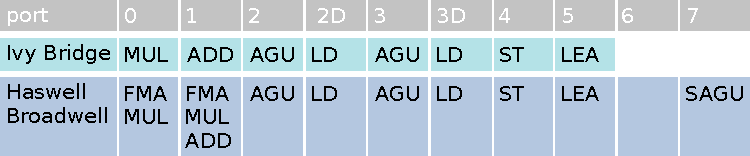
\includegraphics[width=0.49\textwidth,clip=true]{images/IntelMicroArchPorts}
%  \caption{Ports and associated execution units of Intel microarchitectures.
%Only the units relevant for this paper are shown.}
%  \label{fig:ports}
%\end{figure}

The duration of the in-core execution depends on the core's architecture.
For HSW-S it's the Haswell microarchitecture.
The superscalar design has several ports with different execution units for
different types of instructions, shown as part of Figure~\ref{fig:hsw-microarch}.
Instructions scheduled to different ports run independently.
The instruction scheduler takes care that no data dependencies are violated.

\begin{figure}[t]
  \centering
  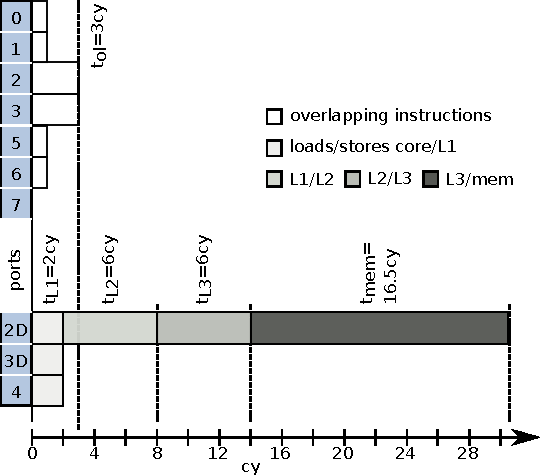
\includegraphics[width=0.42\textwidth,clip=true]{images/ecm-hsw-daxpy}
  \caption{Run time contributions of different execution ports and cache/memory
hierarchy levels for eight iterations of the daxpy kernel on HSW-S (Haswell micro-architecture). It seems that the simple AGU on port~$7$ is not used and all the addresses are generated on ports~$2$ and~$3$.}
  \label{fig:daxpy:ecm}
\end{figure}

\begin{figure}[t]
  \centering
  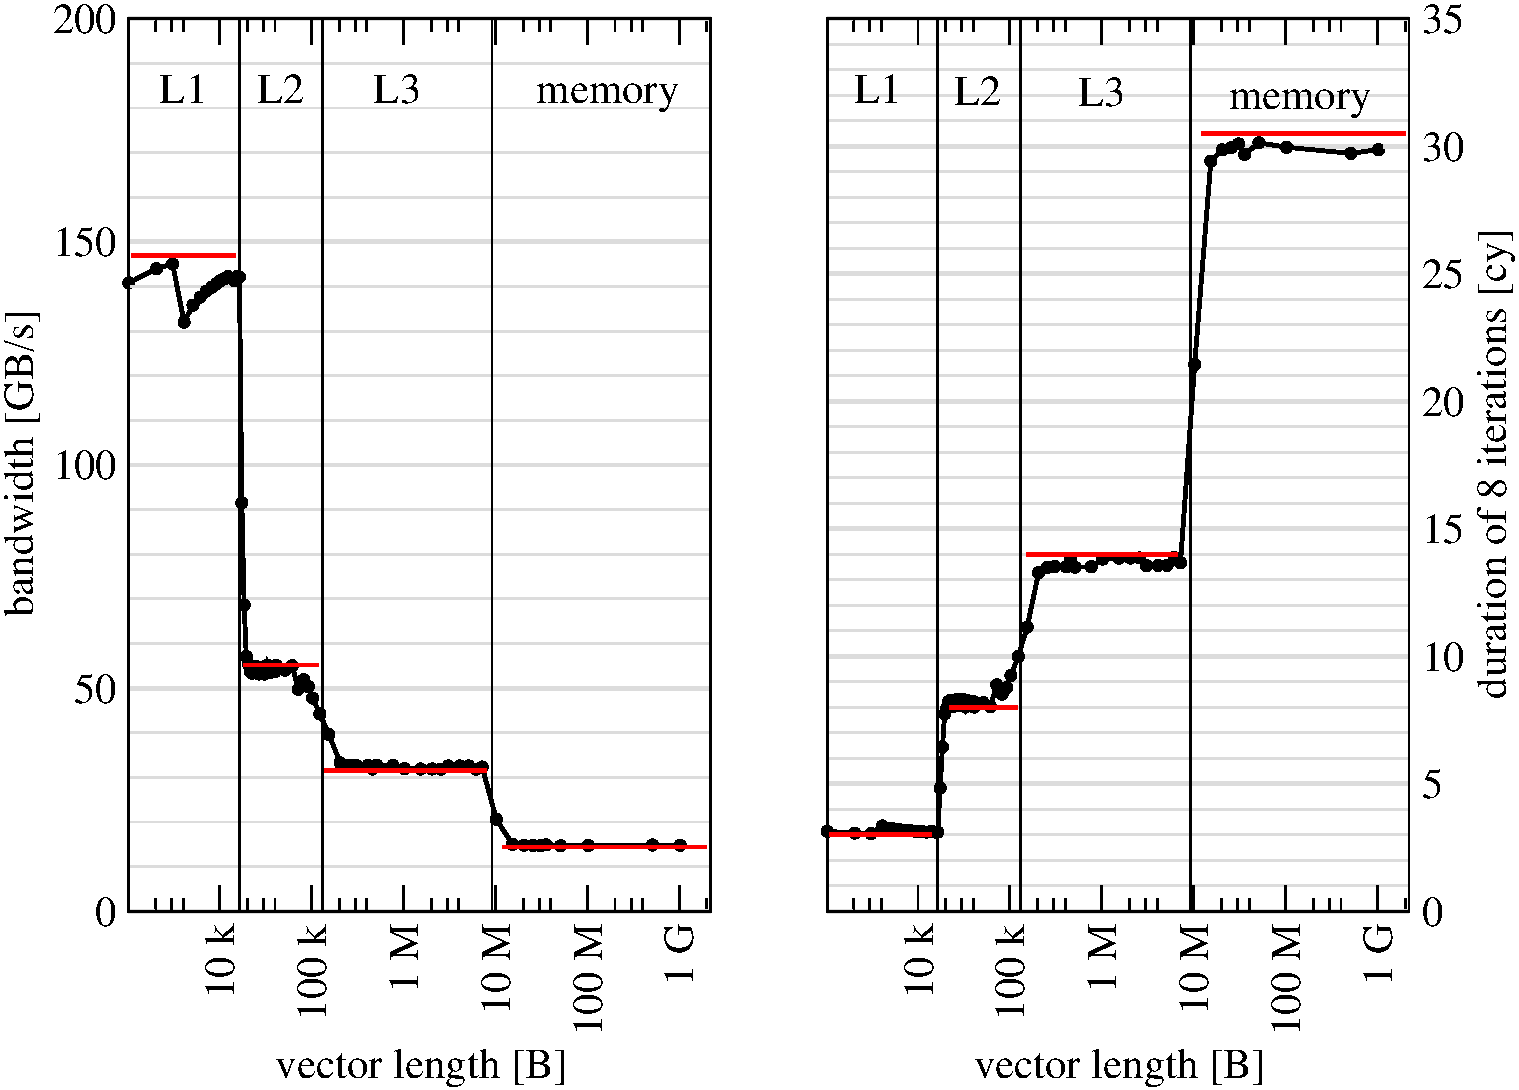
\includegraphics[width=0.60\textwidth,clip=true]{images/daxpy-bw-hasep1-f-2_3-w-cy}
   \caption{Memory bandwidth (left) and duration in CPU cycles of 8 iterations, i.\,e.,\ two iterations of the
compiler generated loop (right), for the daxpy kernel on HSW-S.
   Measurement (black) and ECM prediction (red).
   As the vectors are getting larger and cannot fit in the higher cache levels, the number of cycles for performing 8 iterations increases, which means the performance decreases.
   Note that the total
working set required for vectors
\protect\texttt{r} and \texttt{l} is twice the AVX vector length.}
  \label{fig:daxpy:perf}
\end{figure}

%We could manually analyze the assembly code of the daxpy kernel and create a
%scheduling of the instructions onto the ports to determine the duration of the
%execution inside the core.
%This is not feasible for complex kernels and often requires internal knowledge
%of the core, which is publicly not available.
%Instead we use Intel's Architecture Code Analyzer (IACA) (\cite{intel-iaca})
%for this task.
%We use the tool's throughput mode, where it is assumed that iterations of the
%loop are independent and can overlap due to the out-of-order engine.
%Further we assume no pipeline bubbles of the different ports.
Haswell can perform two loads (port $2D$ and $3D$) and one store (port $4$) of
sizes up to $32$\,B at the same time~(\cite{agner-2016-11-3}).
This constellation requires the store address to be simple addressing as only in
this case the address generation unit (AGU) on port~$7$ can be used.
% Effectively this boils down to either two loads or one load and store.
%
For floating point operations relevant, it hosts two FMA units (port 0 and
1) two MUL units (port 0 and 1), and one ADD unit (port 1).

Under this considerations two iterations of the compiled loop would require $1$\,cy
for the FMA (port $0$ and $1$), $2$\,cy for the four AVX loads (port $2$ and $3$),
and $2$\,cy for the four AVX stores (port $4$).
$6$ addresses need to be generated.
This takes $2$\,cy, if the simple AGU on port $7$ is used.
Instructions regarding index counter increments are for this case negligible, hence we ignore them.
The distribution of the instructions over the ports is found in Figure~\ref{fig:daxpy:ecm}.

For the ECM model the duration of the execution inside the core is split into
two categories.
The first one comprises only data movement between registers and L1 cache,
i.\,e.\ loads, stores occurring and address generation.
The second category consists of the rest, which can possibly overlap with the
loads and stores, like arithmetic, logic.
%We classify the ports into arithmetic/logic (port $0$, $1$, $5$, and $6$) and
%data movement (port $2$, $3$, $4$, and $7$).
The maximum duration $t_\text{L1}$ of the first class (port $2$, $3$, $4$, and $7$) is
\be
  t_\text{L1} = 2\,\cyw.
\ee
The maximum duration of the latter class (port $0$, $1$, $5$, and $6$), $t_\text{ol}$, is
\be
  t_\text{ol} = 1\,\cyw
\ee
%
(normalized to eight iterations) as the maximum duration on the ports overlapping with data
movements.
%
%Note that the compiler uses simple addressing for store addresses, which
%according to IACA will utilize the simple AGU on port~$7$.
%
%
The performance $P_\text{L1}$, when all data are fetched from L1, is then
computed as 
%
\be
  P_\text{L1} = \frac{W}{\max(t_\text{ol}, t_\text{L1})} f,
\ee
%
where $W$ denotes the loop specific work performed and $f$ clock
frequency of the core.
For this loop with $W=192$\,B and $f=2.3$\,GHz we have $P_\text{L1} =
220.8$\,GB/s.
Figure~\ref{fig:daxpy:perf} shows ECM prediction and measured performance for DAXPY kernel of various vector lengths. The graph on the left shows performance and the graph on the right number of CPU cycles needed to perform 8 iterations of the loop. We can see that larger vectors that do not fin in L1 cache and need to be stored in L2 or L3 cache or even the main memory require more cycles, which results in worse performance.
%Measurements shown in Figure~\ref{fig:daxpy:perf} reveal that only around
The measurements for L1 cache reveal that only around
$145$\,GB/s are reached.
If the simple AGU on port~$7$ is not used, the store addresses are
generated by the two remaining AGUs.
This causes $t_\text{ol}$ to be increased by $1$\,\cyw{} and becoming the new
bottleneck.
This results in a corrected
%
\be
   t_\text{ol} = 3\,\cyw
\ee
%
with $P_\text{L1} = 147.2$\,GB/s, which is in line with the measurements as shown in Figure~\ref{fig:daxpy:perf}.


Modeling the performance when data reside in different cache levels from L1
requires analyzing data transfers between these levels.
For daxpy this is straightforward as vectors \verb'r' and \verb'l' are
streamed from/to memory and no cache reuse takes place.
Throughout the cache/memory hierarchy we transfer between each cache level three 
cache lines (cl) for each iteration: load $1$\,cl of \verb'l', load $1$\,cl of
\verb'r', and store $1$\,cl of \verb'r'.

Transferring a cache line between L1/L2 and L2/L3 takes $2$\,cy each.
Hence it takes
%
\be
  t_\text{L2} = 6\,\text{cy} \qquad \text{and} \qquad t_\text{L3} = 6\,\text{cy}
\ee
%
to transfer our three cache lines, respectively.
For computing the performance $P_\text{L2}$ and $P_\text{L3}$, when data resides
in the L2 or L3 cache, respectively, we have to add $t_\text{L2}$ and $t_\text{L3}$
to the duration of the data path, as on the considered Intel architectures data
transfers seem be be serialized when streaming accesses occur.\footnote{This need
not be the actual implementation inside the architecture; it only resembles
the observation and can be different on other architectures.}
The performance is then
%
\begin{align}
  P_\text{L2} &= \frac{W}{\max(t_\text{ol}, t_\text{L1} + t_\text{L2})} f, \\
  P_\text{L3} &= \frac{W}{\max(t_\text{ol}, t_\text{L1} + t_\text{L2} +
t_\text{L3})} f.
\end{align}
%
In our case $P_\text{L2} = 55.2$\,GB/s and $P_\text{L3} = 31.5$\,GB/s.
%

%How many cache lines per cycle can be transferred between L3 and memory could
%theoretically be obtained by taking the nominal memory bandwidth into account.
%However, this bandwidth is practically never reached and depends strongly on the
%access pattern used.
%This is caused by the organization of the memory subsystem, where e.\,g.\ banking
%conflicts and DRAM page misses incur performance.
%With detailed knowledge about the internals of the (closed IP) memory controller
%(scheduling strategies, thresholds for strategy switching, ...) and DRAM modules
%this could also be modeled, which is far from being trivial~\cite{jacob-2007}.
%As this is beyond the scope of the ECM model typically a micro benchmark
%resembling the used access pattern by the code under investigation is used
%to measure the attainable bandwidth and use it as input for the model.
%%
%For this model we use \textsc{McCalpin's} STREAM copy
To determine the memory bandwidth we use \textsc{McCalpin's} STREAM copy
benchmark (\cite{mccalpin-1995}) which achieves (without nontemporal stores and
including the write allocate) a bandwidth of $\approx 26.9$\,GB/s when all cores
of a cluster are utilized\footnote{When Cluster-on-Die (COD) is enabled, the cores are split into two NUMA domains. The HSW-S processor has 14 cores, that are split in two NUMA domains, each with 7 cores.}.
With the core's clock frequency of $2.3$\,GHz it takes $5.5$\,cy to transfer one
cache line between L3 cache and memory.
Transferring our three cache lines between these two levels takes then
%
\be
  t_\text{mem} = 16.5\,\text{cy}.
\ee
%
The performance $P_\text{mem}$, when every vector is streamed from memory, is then
%
\be
  P_\text{mem} = \frac{W}{\max(t_\text{ol}, t_\text{L1} + t_\text{L2} +
t_\text{L3} + t_\text{mem})} f.
\ee
%
This leads to $P_\text{mem} = 14.5$\,GB/s. 

\subsection{Indirect DAXPY}
\label{sec:ecm-indirect-daxpy}

Indirect DAXPY is similar to the code analyzed in section \ref{sec:epm}, with the difference of indirect access \verb|idx| to the vector \verb|r|.

%
\begin{lstlisting}
for (int i = 0; i < N; ++i) 
  r[idx[i]] +=  s * l[i];
\end{lstlisting}
%
The vectors \verb'r' and
\verb'l' are double-precision floating point vectors with \verb'N' elements
each. 
The \verb'idx' vector contains $4$~B integers.
Furthermore \verb's' is a scalar double precision floating point variable.
%
The code is 4-way unrolled and by the compiler, when
optimizations are turned on and target ISA is AVX2 and FMA3. One iteration
over this newly formed loop now performs 4 scalar iterations. The code snipped
from above effectively becomes
%
\begin{lstlisting}
for (int i = 0; i < N; i += 4)
{
  r[idx[i  ]] += s * l[i  ];
  r[idx[i+1]] += s * l[i+1];
  r[idx[i+2]] += s * l[i+2];
  r[idx[i+3]] += s * l[i+3];
}
\end{lstlisting}
%
For the ECM model we determine the duration of the execution of the code inside
the core under the assumption all operands reside in L1 cache.

\begin{figure}[t]
  \centering
  \includegraphics[width=0.56\textwidth,clip=true]{images/ecm-hsw-daxpy-indirect}
  \caption{Run time contributions of different execution ports and cache/memory
hierarchy levels for eight iterations of the indirect daxpy kernel on HSW-S (Haswell micro-architecture).}
  \label{fig:daxpy-indirect:ecm}
\end{figure}

\begin{figure}[t]
  \centering
  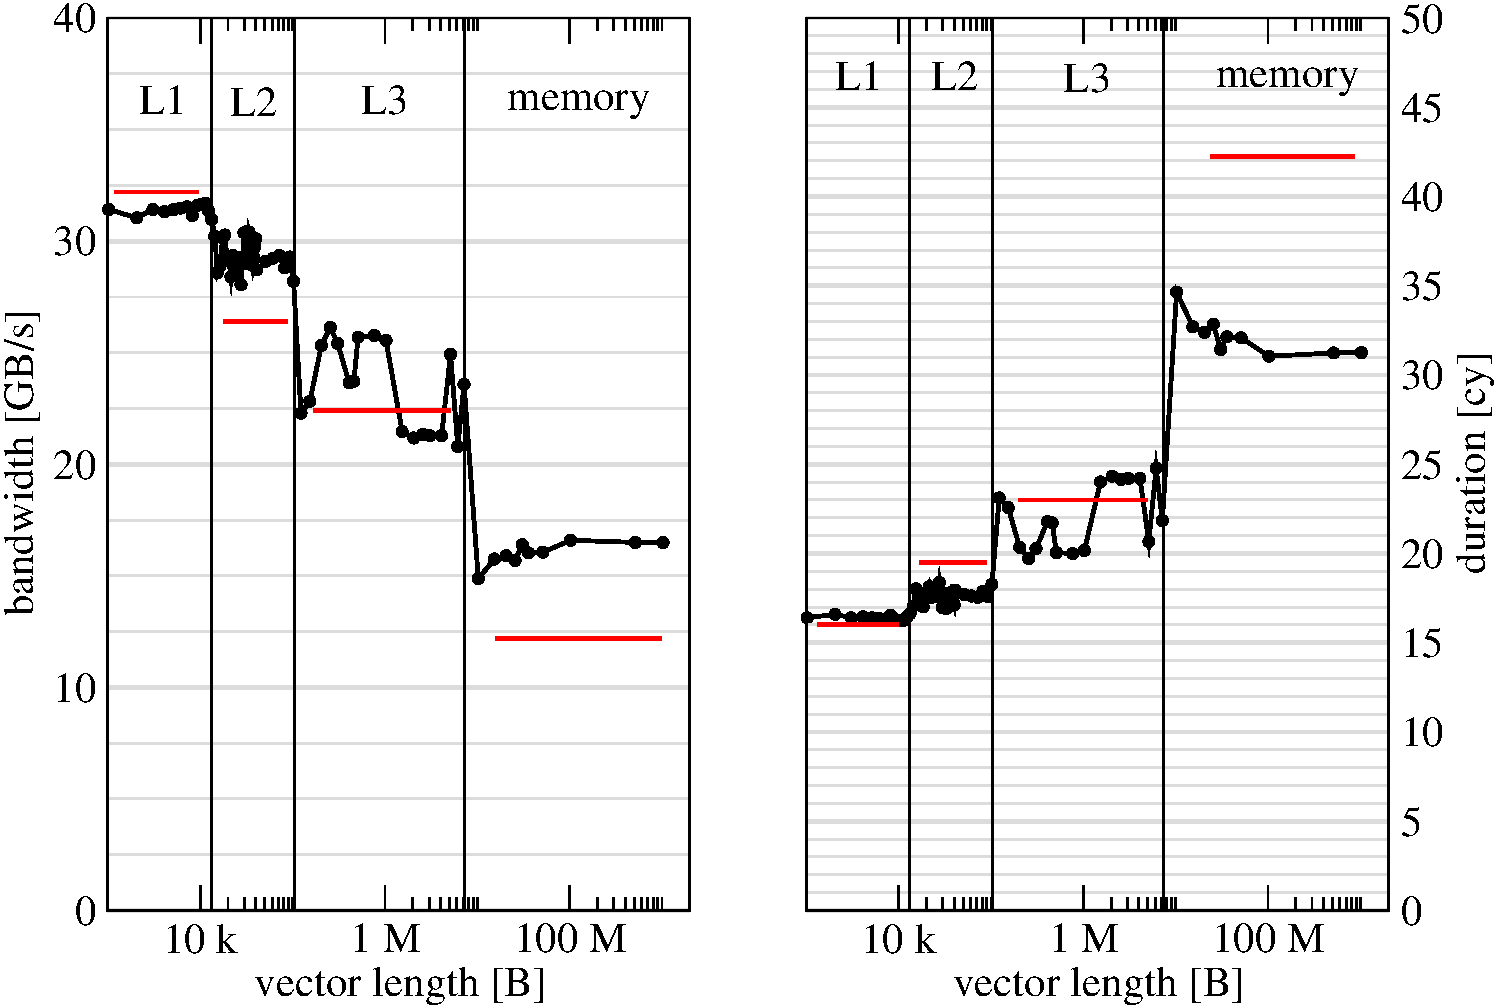
\includegraphics[width=0.60\textwidth,clip=true]{images/daxpy-indirect-bw-hasep1-f-2_3-w-cy}
   \caption{Memory bandwidth (left) and duration in CPU cycles of 8 iterations, i.\,e.,\ two iteration of the
compiler generated loop (right), for the indirect daxpy kernel on HSW-S.
   Measurement (black) and ECM prediction (red).
   As the vectors are getting larger and cannot fit in the higher cache levels, the number of cycles for performing 8 iterations increases, which means the performance decreases.}
  \label{fig:daxpy-indirect:perf}
\end{figure}

Eight iterations of the loop (or two iterations of the unrolled loop) require
sixteen $8$\,B loads (\verb|r[:]| and
\verb|l[:]|), eight $4$\,B loads (\verb'idx[:]'), eight
$8$\,B stores (\verb'r[:]'), and $32$ address generations.
Furthermore eight scalar fused-multiply-adds are used. 
We define the work performed by eight iterations of the loop (or two iterations of compiler unrolled loop) to be $W =
224$\,B.

How long the execution takes depends on the underlying architecture. 
In order to determine this, we take a look at the Intel Haswell
microarchitecture in Fig.~\ref{fig:hsw-microarch}.
The super-scalar design has several ports with different execution units for
different types of instructions.
Instructions scheduled to different ports run independently.
The instruction scheduler takes care that no data dependencies are violated.
Instructions inside ports are pipelined, but only one instruction per port can
be issued per cycle.
Haswell can perform two loads (port $2D$ and $3D$) and one store (port $4$) of
sizes up to $32$\,B at the same time~(\cite{agner-2016-11-3}).
This constellation requires the store address to be simple addressing as only in
this case the address generation unit (AGU) on port~$7$ can be used.
% Effectively this boils down to either two loads or one load and store.
%
For floating point operations relevant, it hosts two FMA units (port 0 and
1) two MUL units (port 0 and 1), and one ADD unit (port 1).

Under this considerations two iterations of the compiled loop would require $4$\,cy
for the FMA (port $0$ and $1$), $12$\,cy for the twenty four loads (port $2$ and $3$),
and $8$\,cy for the eight stores (port $4$).
$32$ addresses need to be generated. We assume the simple AGU on port $7$ is not used, as we observed for DAXPY (section \ref{sec:epm}). Generating all $32$ addresses on AGUs on ports $2$ and $3$ requires $16$\,cy.
Instructions regarding index counter increments are for this case negligible, hence we ignore them.
%From the $32$ address generation four are simple an can run on the simple AGU on
%port $7$ requiring $4$\,cy, whereas the remaining $28$ addresses are handled in
%$14$\,cy due to two AGUs on port $3$ and $4$.
We assume that the out-of-order engine can fill bubbles in the pipelines of the
different ports as the loop iterations are independent of each other.
We classify the ports into arithmetic/logic (port $0$, $1$, $5$, and $6$) and
data movement (port $2$, $3$, $4$, and $7$). 
The maximum duration $t_\text{ol}$ of the first class of ports is 
%
\be
  t_\text{ol} = \max(4\,\cyw, 4\,\cyw, 6\,\cyw, 6\,\cyw)
= 6\,\cyw
\ee
%
and the maximum duration of the data movement ports $t_\text{L1}$ which
load/store data from/to L1 is
\be
%  t_\text{L1} = \max(12\,\cyw, 14\,\cyw, 8\,\cyw, 4\,\cyw) =
  t_\text{L1} = \max(16\,\cyw, 16\,\cyw, 8\,\cyw, 0\,\cyw) =
16\,\cyw.
\ee
%
% for the duration of the data transfers between core and L1 cache.
%
The performance $P_\text{L1}$, when all data is fetched from L1, is then computed as 
%
\be
  P_\text{L1} = \frac{W}{\max(t_\text{ol}, t_\text{L1})} f,
\ee
%
where $W$ denotes the loop specific work performed and $f$ clock frequency of the core.
For this loop with $W=224$\,B and $f=2.3$\,GHz we have $P_\text{L1} =
32.2$\,GB/s,
%On HSW1 only $\approx 31$\,GB/s, i.\,e.\ 80\,\% of the predicted
%performance are achieved for this loop, shown in
which is in line with the measurements in
Figure~\ref{fig:daxpy-indirect:perf}.

Modeling the performance when data resides in different cache levels from L1
requires to analyse the data transfers between these levels.
In this case this is straight forward as vector \verb'r', \verb'l', and
\verb'idx' are streamed from/to memory and no cache reuse takes place.
Throughout the cache/memory hierarchy we transfer between each cache level
$224$\,B $= 3.5$\,cl (cache lines) for each iteration: load $64$\,B of
\verb'l', load $64$\,B of \verb'r', load $32$\,B of \verb'idx' and store $64$\,B
of \verb'r'.

Transferring a cache line between L1/L2 and L2/L3 takes $1$\,cy (\cite{intel-orm-2016}). Hence it takes
%
\be
  t_\text{L2} = 3.5\,\cyw\ \text{and}\ t_\text{L3} = 3.5\,\cyw
\ee
%
to transfer our $224$\,B.
For computing the performance $P_\text{L2}$ and $P_\text{L3}$, when data resides
in L2 or L3 cache, respectively, we
have to add $t_\text{L2}$ and $t_\text{L3}$ to the duration of the data path, as on the considered
Intel architectures data transfers seem be be serialized when streaming accesses
occur\footnote{This need not to be the actual implementation inside the
architecture, it only resembles the observation and can be different on other
architectures.}.
The performance is then
%
\begin{align}
  P_\text{L2} &= \frac{W}{\max(t_\text{ol}, t_\text{L1} + t_\text{L2})} f, \\
  P_\text{L3} &= \frac{W}{\max(t_\text{ol}, t_\text{L1} + t_\text{L2} +
t_\text{L3})} f.
\end{align}
%
%In our case $P_\text{L2} = 29.4$\,GB/s and $P_\text{L3} = 18.2$\,GB/s.
In our case $P_\text{L2} = 26.4$\,GB/s and $P_\text{L3} = 22.4$\,GB/s.
%

How many cache lines per cycle can be transferred between L3 and memory could
theoretically be obtained by taking the nominal memory bandwidth into account.
However, this bandwidth is practically never reached and depends strongly on the
access pattern used.
This is caused by the organization of the memory subsystem, where e.\,g.\ banking
conflicts and DRAM page misses incur performance.
With detailed knowledge about the internals of the memory controller
(scheduling strategies, thresholds for strategy switching, ...) and DRAM modules
this could also be modeled, which is far from being trivial (\cite{jacob-2007}).
As this is beyond the scope of the ECM model typically a micro benchmark
resembling the used access pattern by the code under investigation is used
to measure the attainable bandwidth and use it as input for the model.
%
For this model we use \textsc{McCalpin's} STREAM copy
benchmark~(\cite{mccalpin-1995}) which achieves (without nontemporal stores and
including the write allocate) a bandwidth of $\approx 26.9$\,GB/s when all cores
of a cluster are utilized.
With the core's clock frequency of $2.3$\,GHz it takes $5.5$\,cy to transfer one
cache line between L3 cache and memory.
Transferring our $224$\,B between these to levels takes
%
\be
%  t_\text{mem} = 9.625\,\cyw.
  t_\text{mem} = 19.25\,\cyw.
\ee
%
The performance $P_\text{mem}$, when every vector is streamed from memory, is then
%
\be
  P_\text{mem} = \frac{W}{\max(t_\text{ol}, t_\text{L1} + t_\text{L2} +
t_\text{L3} + t_\text{mem})} f.
\ee
%
%This leads to $P_\text{mem} = 10.2$\,GB/s. 
This leads to $P_\text{mem} = 12.2$\,GB/s. 
Which is about $23\,\%$ less than the achieved performance on HSW-S architecture. While the ECM prediction of the DAXPY kernel is in line with measurements, in case of indirect DAXPY kernel the ECM model underestimates the measured performance. The ECM model was developed and studied mostly for vectorized codes. As indirect DAXPY kernel is not vectorized, it would require further investigation.

%% The required information on the hardware capabilities can be obtained from the
%% data sheets of the vendors or measured via micro-benchmarks.
%% For good estimates regarding achievable memory bandwidth a benchmark which
%% exhibits the same access pattern as the code under investigation is preferable.
%% %
%% In our case primarily the nonzeros from matrix $L$ out of the \vlnz{}
%% array are loaded from memory.
%% Hereby we neglect, that for each panel also the indices into the right hand side
%% $r$ must be loaded. 
%% This seems to be a fair assumption for matrices with large panel sizes, like the
%% dense\footnote{MW: here already reference to the dense matrix} matrix with $n_p = 80$.
%% Here only for the panel's first column, indices must be loaded from memory
%% and can be $79$ times reused.
%% Further we ignore that during forward substitution stores to $r$ occur.
%% %
%% The most simple benchmark, which resembles this behavior, is linearly reading
%% from memory.
%% We accomplish this by summing up the elements of a vector $a$ which is large
%% enough to reside in memory: \texttt{s = s + a[i]}.
%% Note that the single core bandwidth for read only is below the STREAM copy
%% bandwidth (\texttt{a[i] = b[i]}).
%% Here \textsc{McCalpin} identifies limited concurrency as the
%% bottleneck\footnote{Comment of \textsc{McCalpin} in the Intel Forum found under
%% \texttt{http://software.intel.com/en-us/forums/topic/456184}.}.
%% However in the saturated case a higher bandwidth compared to STREAM copy is
%% achieved.
%% Through an $n$-way unrolling over columns
%% (described in section~\ref{sec:pm:dt:wu}) there are effectively $n$ concurrent
%% read streams for each core.
%% For simplicity we ignore the fact that with $n > 1$ possibly the attainable
%% bandwidth decreases.
%% %
%% Table~\ref{tab:hw} contains all the ECM model parameters used for the different
%% hardware systems.
%% 
